\section{Evidence from Binance futures depth}\label{sec:depth}

\subsection{Data and validation}
We use Binance USD-M BTCUSDT perpetual futures from the public archive: one-minute klines with taker-buy volume, \texttt{bookDepth} snapshots of cumulative depth within $\pm1$--$5\%$ of the mid at about 30-second intervals, and open interest from \texttt{metrics}. Depth is available from January 2023. No liquidation archive is available for this period, so we do not test liquidations.

Validation rules were fixed before analysis. A snapshot is kept if (V1) all of the $\pm1,2,5\%$ bands are present, (V2) depth is monotone in distance on each side, (V3) the implied average price at $\pm1\%$ is within 3\% of the one-minute close, and (V4) it is not part of a run of more than ten identical snapshots; (V5) a day is kept if at least 80\% of its minutes have a valid snapshot.

\begin{table}[t]\centering\small
\begin{threeparttable}
\caption{Depth data validation}\label{tab:d2}
\begin{tabular}{lr}
\toprule
Days requested (January 2023 -- October 2026) & 1{,}386\\
Days passing validation & 1{,}329\\
Snapshots examined & 3{,}897{,}951\\
\quad dropped by V1 (missing bands) & 0\\
\quad dropped by V2 (non-monotone) & 0\\
\quad dropped by V3 (implied price off by $>3\%$) & 98{,}080\\
\quad dropped by V4 (stuck feed) & 95{,}954\\
Failed periods & April 16 -- May 19, 2025; October 10--15, 2025\\
Training days used (2023--2024) & 718\\
\bottomrule
\end{tabular}
\begin{tablenotes}\footnotesize\item All files verified against published SHA-256 checksums. The 2025 failures coincide with archived depth that is misaligned with prices; the October 10, 2025 crash day is therefore unusable. \end{tablenotes}
\end{threeparttable}
\end{table}

\subsection{Structural estimates}
On one-minute bars, $p_t$ is the log price in basis points, $u_t$ signed taker flow in million USDT, $d_t=(B_1-A_1)/(B_1+A_1)$ the depth imbalance within 1\% of the mid, and $x_t=p_t-{\rm EMA}_{60}(p_t)$. Day by day we estimate
\begin{align*}
\Delta p_t&=\kappa u_t+\varphi d_{t-1}-(1-a)x_{t-1}+e_t,\\
d_t&=(1-r)d_{t-1}+\varepsilon u_t+e_t,\\
u_t&=(1-\eta)u_{t-1}+\eta q\,x_{t-1}+e_t,
\end{align*}
and form $\hat C_2$, $\hat C_3$ and the implied peak ratio $\max_k\hat h_k/\hat h_0$. The price equation has $\Delta p_t$ on the left, so the EMA filter does not create mechanical persistence. These are reduced-form regressions (flow is contemporaneous), so the estimates describe conditional dynamics rather than causal parameters.

\begin{table}[t]\centering
\begin{threeparttable}
\caption{Day-by-day T6 estimates, Binance BTCUSDT futures, training days 2023--2024}\label{tab:d3}
\small\setlength{\tabcolsep}{4pt}
\begin{tabular}{lccc}
\toprule
Median & All days & Top-decile volatility days & Other days\\
\midrule
$\hat\kappa$ (bp per \$1M) & 0.729 & 0.890 & 0.712\\
$\hat\varphi$ & $-0.051$ & 2.586 & $-0.138$\\
$\hat a$ & 0.970 & 0.980 & 0.969\\
$\hat r$ & 0.059 & 0.122 & 0.056\\
$\hat\varepsilon$ & $-0.0018$ & $-0.0017$ & $-0.0018$\\
$\hat\eta$ & 0.878 & 0.863 & 0.880\\
$\hat q$ & 0.018 & 0.012 & 0.019\\
$\hat C_3$ & $-0.0137$ & $-0.0111$ & $-0.0143$\\
\midrule
Mean $\hat C_3$ & $-0.0165$ & $-0.0167$ & $-0.0165$\\
\quad 95\% CI & [$-0.0176$, $-0.0155$] & [$-0.0219$, $-0.0122$] & [$-0.0175$, $-0.0154$]\\
Share of days $\hat C_3>0$ & 6.5\% & 5.6\% & 6.7\%\\
Share of days $\hat C_2>0$ & 0.8\% & 1.4\% & 0.8\%\\
Median peak ratio & 1.00 & 1.00 & 1.00\\
Days & 718 & 72 & 646\\
\bottomrule
\end{tabular}
\begin{tablenotes}\footnotesize\item One-minute bars. CIs from a day bootstrap. \end{tablenotes}
\end{threeparttable}
\end{table}

Table~\ref{tab:d3} has three findings. First, the market sits on the stable side of the condition: $\hat C_3<0$ on 93.5\% of days, and the median implied response peaks at impact. Second, the depletion coefficient $\hat\varepsilon$ is small and negative: taker buying is followed by slightly more ask-side than bid-side depth within 1\%, so in these re-centred bands the book appears to replenish rather than deplete the side being hit; Section~\ref{sec:fixedgrid} shows that a fixed price grid reverses the sign. With $\hat\varepsilon<0$, $\varphi\varepsilon$ is positive only if $\varphi$ is negative, which it is not on high-volatility days. Third, on high-volatility days depth imbalance moves prices strongly ($\hat\varphi=2.59$) and refill is twice as fast; the depth channel is active, but it works against amplification. The momentum term $\kappa^2\eta q$ is small (about $0.008$ at the medians), far below $(1-a)\kappa\approx0.022$.

\subsection{Does depth carry an overshoot?}
We estimate local projections \citep{jorda2005} of the cumulative price change on flow, $p_{t+k}-p_{t-1}=\beta_ku_t+\text{controls}$, with five lags of returns, flow and depth: (A) total; (B) adding cumulative future flow, which removes order-splitting persistence; and (C) adding cumulative future depth imbalance, which removes the depth channel. Theorem~\ref{thm:peak}\ref{thm:t6} predicts an overshoot ($\max_{k\ge1}\beta_k-\beta_0>0$) in (B) that shrinks in (C).

\begin{figure}[t]\centering
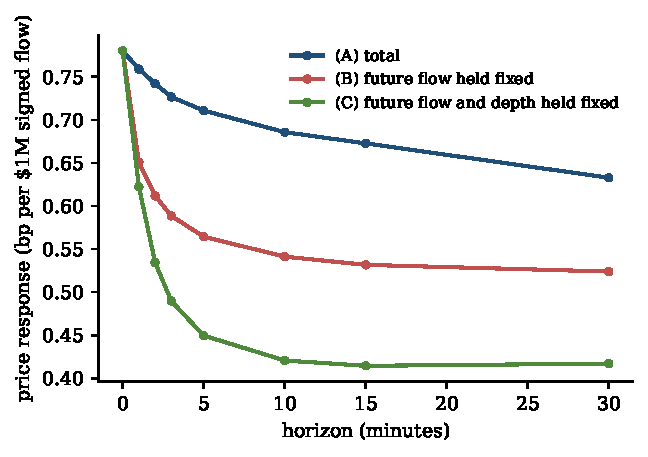
\includegraphics[width=0.6\textwidth]{figs/fig_mediation.pdf}
\caption{Price response to a \$1M flow shock, local projections on 716 training days. (A) total; (B) future flow held fixed; (C) future flow and depth held fixed.}\label{fig:med}
\end{figure}

\begin{table}[t]\centering\small
\begin{threeparttable}
\caption{Local-projection coefficients (bp per \$1M) and overshoots}\label{tab:d4}
\setlength{\tabcolsep}{3.5pt}
\begin{tabular}{lccccccccc}
\toprule
Minutes & 0 & 1 & 2 & 3 & 5 & 10 & 15 & 30 & Overshoot\\
\midrule
(A) total & 0.780 & 0.759 & 0.742 & 0.727 & 0.711 & 0.686 & 0.673 & 0.633 & $-0.021$\\
 & & & & & & & & & [$-0.027$, $-0.015$]\\
(B) flow fixed & 0.780 & 0.651 & 0.612 & 0.589 & 0.564 & 0.541 & 0.532 & 0.524 & $-0.129$\\
 & & & & & & & & & [$-0.134$, $-0.124$]\\
(C) flow, depth fixed & 0.780 & 0.622 & 0.534 & 0.490 & 0.450 & 0.421 & 0.414 & 0.417 & $-0.158$\\
 & & & & & & & & & [$-0.164$, $-0.152$]\\
\bottomrule
\end{tabular}
\begin{tablenotes}\footnotesize\item 716 training days; day bootstrap. \end{tablenotes}
\end{threeparttable}
\end{table}

There is no overshoot (Figure~\ref{fig:med}, Table~\ref{tab:d4}). The overshoot statistic is negative in every version. Holding depth fixed makes the response decay faster, consistent with depth that partly sustains the price move but never pushes it past impact.

\subsection{Pre-registered out-of-sample test}
Before opening the test period we registered the specification (SHA-256 \texttt{d95212187ae4\ldots}): hourly blocks (06:00--23:00 UTC); $\hat C_3$ estimated from the previous six hours and winsorized at training percentiles; outcome the next hour's maximum adverse excursion (MAE, bp); controls for realized volatility (1 and 6 hours), absolute return, flow imbalance, volume, depth, imbalance and open-interest change; OLS on 2023--2024 and evaluation on 2025--2026. Success required a one-sided Clark--West $p<0.05$ \emph{and} a day-block bootstrap 95\% CI for $\Delta R^2$ excluding zero. Secondary candidates and outcomes are Holm-adjusted. The test set was opened once. An audit that scrambles all data from $t$ onward left every feature unchanged in 30 of 30 trials.

\begin{table}[t]\centering
\begin{threeparttable}
\caption{Out-of-sample test, 2025--2026 (train 12,896 hours, test 10,979 hours)}\label{tab:d8}
\small\setlength{\tabcolsep}{4pt}
\begin{tabular}{llccc}
\toprule
Outcome & Candidate & $\Delta R^2$ (pts) [95\% CI] & $\Delta$AUC [95\% CI] & Holm $p$\\
\midrule
MAE (primary) & $\hat C_3$ & $+0.018$ [$-0.100$, $+0.132$] & $+0.0001$ [$-0.0009$, $+0.0012$] & ---\\
MAE & peak ratio & $+0.010$ [$+0.001$, $+0.019$] & $+0.0001$ [$-0.0000$, $+0.0002$] & 0.032\\
OI drop & $\hat C_3$ & $-0.045$ [$-0.095$, $-0.003$] & $-0.0049$ [$-0.0083$, $-0.0016$] & 0.787\\
OI drop & peak ratio & $+0.102$ [$+0.061$, $+0.231$] & $-0.0014$ [$-0.0067$, $+0.0037$] & $<0.001$\\
Depth collapse & $\hat C_3$ & $+0.181$ [$-0.156$, $+0.484$] & $+0.0071$ [$+0.0041$, $+0.0105$] & $<0.001$\\
Depth collapse & peak ratio & $+0.159$ [$+0.094$, $+0.234$] & $+0.0009$ [$+0.0004$, $+0.0014$] & $<0.001$\\
\bottomrule
\end{tabular}
\begin{tablenotes}\footnotesize\item Primary: Clark--West one-sided $p=0.023$, but the $\Delta R^2$ CI contains zero, so the pre-registered test fails. Baseline $R^2$ for MAE is 0.293; baseline AUC 0.812. \end{tablenotes}
\end{threeparttable}
\end{table}

The primary test fails (Table~\ref{tab:d8}): $\hat C_3$ adds $0.018$ percentage points of out-of-sample $R^2$ with a confidence interval that includes zero. Some secondary effects are statistically significant after Holm correction, notably for depth collapse, but they are economically negligible: no candidate adds more than $0.2$ points of $R^2$ or $0.01$ of AUC.

\paragraph{A volatility flag does better.} We set two flags on training data, each to flag 10\% of hours: high $\hat C_3$ and high realized volatility. On the 909 tail hours of the test period (MAE above the training 90th percentile), the $\hat C_3$ flag has precision $8.6\%$ and recall $19.5\%$; the volatility flag has precision $38.1\%$ and recall $37.1\%$; the union has precision $16.3\%$ and recall $49.4\%$. The unconditional tail rate is about 10\%, so the $\hat C_3$ flag is no better than chance.

\subsection{Crash events}
For each event day we compute $\hat C_3$ hour by hour and its percentile in the training distribution during the three hours before the worst hour (Figure~\ref{fig:events}, Table~\ref{tab:d9}). $\hat C_3$ was elevated before these events but stayed negative throughout, and three events are not a test.

\begin{table}[t]\centering\small
\begin{threeparttable}
\caption{Event days}\label{tab:d9}
\begin{tabular}{lcccc}
\toprule
Event & Worst hour & Worst MAE & $\hat C_3$ percentile, & OI change\\
 & (UTC) & (bp) & 3 hours before & in worst hour\\
\midrule
SVB, 2023-03-11 & 7 & 214.8 & 82 & $+2.5\%$\\
Yen carry unwind, 2024-08-05 & 13 & 724.0 & 93, 84, 83 & $-0.8\%$\\
Tariff shock, 2025-04-07 & 14 & 357.8 & 97, 98, 38 & $+3.1\%$\\
2025-10-10 & \multicolumn{4}{c}{no valid depth data}\\
\bottomrule
\end{tabular}
\begin{tablenotes}\footnotesize\item SVB has one valid hour before its worst hour. \end{tablenotes}
\end{threeparttable}
\end{table}

\begin{figure}[t]\centering
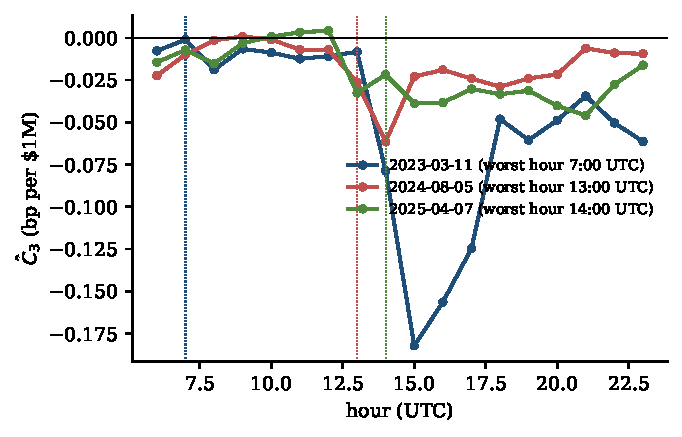
\includegraphics[width=0.6\textwidth]{figs/fig_events.pdf}
\caption{Hourly $\hat C_3$ on three event days (UTC). Values stay below zero, the amplification threshold.}\label{fig:events}
\end{figure}

\section{Evidence from spot prices}\label{sec:spot}

\subsection{A unit-free amplification statistic}
The earlier version measured amplification by the norm of powers of a VAR(1) operator on (price deviation, flow), estimated over ten-minute windows of one-second Binance spot data. That norm depends on the units of the state: multiplying prices by 10 and dividing flow by 1,000 changed the raw norm from $8.73$ to $86{,}731$ on the same window. Proposition~\ref{prop:invariance} explains why: state norms are not invariant to coordinates. We therefore standardize the state, $\tilde J=D^{-1}\hat JD$ with $D={\rm diag}({\rm sd}\,x,{\rm sd}\,f)$, and use $M_{\rm std}=\max_k\|e_x^\top\tilde J^k\|$, which is invariant to units (verified). We also report the price-to-price amplification $A_{xx}=\max_k|(\hat J^k)_{11}|$ and a delayed-peak statistic ${\rm hump}=\max_k|(\hat J^k)_{12}|/|\hat J_{12}|$.

\subsection{Crash days and a no-feedback null}
We study five crash days: May 19, 2021; LUNA, May 9, 2022; FTX, November 8, 2022; SVB, March 11, 2023; and August 5, 2024. Windows are selected \emph{ex ante} (previous ten minutes in the top volatility decile), and for comparison by outcome (the ten largest absolute returns). A no-feedback null keeps each window's real flow, generates prices with no feedback, $\Delta p=\hat\kappa f+\hat\sigma e$, and pushes them through the identical pipeline.

\begin{table}[t]\centering\small
\begin{threeparttable}
\caption{Unit-free amplification on crash days and the no-feedback null}\label{tab:spotnull}
\begin{tabular}{lccccc}
\toprule
Event & Windows (ex ante) & Mean $M_{\rm std}$ & Null 99th pct & $p$ (vs null) & Outcome-selected mean\\
\midrule
May 2021 & 142 & 1.0000 & 1.00002 & 1.00 & 1.0000\\
LUNA 2022 & 57 & 1.00008 & 1.00006 & 0.039 & 1.00045\\
FTX 2022 & 49 & 1.0000 & 1.00029 & 1.00 & 1.0000\\
SVB 2023 & 6 & 1.00006 & 1.00025 & 0.059 & 1.00032\\
Aug 2024 & 108 & 1.0000 & 1.00007 & 1.00 & 1.0000\\
\bottomrule
\end{tabular}
\begin{tablenotes}\footnotesize\item Ten-minute windows of one-second bars. The median hump statistic is 1.000 in every event and its null $p$-value is 1.00. In the ordinary 2021--2023 panel, 0.2\% of windows have $A_{xx}>1$ and the 95th percentile of $M_{\rm std}$ is 1.0000; a handful of near-singular windows produce very large values, so ordinary-window means are not informative. \end{tablenotes}
\end{threeparttable}
\end{table}

Only LUNA exceeds the null, by less than $0.01\%$ (Table~\ref{tab:spotnull}). Outcome-selected windows give only marginally larger values ($\le1.0005$). Stress-window means exceed the ordinary 95th percentile in two events, by amounts of the same size. The pre-registered gate fails: unit-free transient amplification in spot data is indistinguishable from one and from the pipeline null. Varying the EMA span (60, 120, 300 seconds) and the bar length (1 or 5 seconds) does not change this; crash-day means range from $1.0003$ to $1.18$ across specifications and are never above the corresponding ordinary means.

\subsection{Overshoot with flow held fixed}
Local projections on one-second data give the price response to a \$1M flow shock (Table~\ref{tab:spotlp}). On ordinary days, with future flow held fixed, there is a small, short-lived overshoot of $+0.248$ [$0.133$, $0.376$] bp per \$1M, peaking at two seconds and decaying after. On crash days the flow-fixed overshoot is negative, $-0.277$ [$-0.528$, $-0.042$]. The large total overshoots ($+0.91$ ordinary, $+2.40$ crash) disappear when future flow is held fixed: they come from order splitting, not from the book.

\begin{table}[t]\centering\small
\begin{threeparttable}
\caption{Spot local projections (bp per \$1M)}\label{tab:spotlp}
\setlength{\tabcolsep}{3.5pt}
\begin{tabular}{lcccccccccc}
\toprule
Seconds & 0 & 1 & 2 & 5 & 10 & 20 & 30 & 60 & 120 & 300\\
\midrule
Ordinary, total & 5.86 & 6.28 & 6.53 & 6.60 & 6.69 & 6.77 & 6.67 & 6.49 & 6.39 & 5.92\\
Ordinary, flow fixed & 5.86 & 6.02 & 6.11 & 5.90 & 5.68 & 5.26 & 4.86 & 4.16 & 3.37 & 1.99\\
Crash, total & 6.69 & 6.85 & 6.92 & 7.13 & 7.75 & 8.20 & 8.46 & 8.20 & 9.09 & 8.96\\
Crash, flow fixed & 6.69 & 6.41 & 6.28 & 5.99 & 5.95 & 5.46 & 5.02 & 3.88 & 3.10 & $-0.08$\\
\bottomrule
\end{tabular}
\begin{tablenotes}\footnotesize\item\end{tablenotes}
\end{threeparttable}
\end{table}

\subsection{Pre-registered predictive test}
Before opening 2024, we registered (SHA-256 \texttt{b1fd7f8e\ldots}) a test of whether pre-window amplification predicts the next ten minutes' MAE beyond volatility and flow controls, on non-overlapping 30-minute blocks (train 2021--2023, 3,307 blocks; test 2024, 1,104 blocks). It does not: $\Delta R^2=-0.023$ points [$-0.056$, $-0.002$], Clark--West $p=0.966$, AUC $0.822$ in both models. A random feature with the same autocorrelation gives $\Delta R^2=-0.020$ points, the same as the candidate. Leave-one-year-out fits within the training period are unstable (the 2023 fold gives a very large negative $\Delta R^2$ because of outlying candidate values), so the null result does not depend on one year being unusual.

The test set was opened three times. The first evaluations stopped on a numerical error from degenerate windows; the fix drops blocks with non-finite features (five blocks) and is the only change, and the registered specification hash is unchanged. A volatility flag again dominates: precision $43\%$ and recall $30\%$ against $3\%$ and $10\%$ for the amplification flag; the difference in recall has a CI of $[-0.37,0.13]$.

